% Generated by scripts/build-paper.py — edit paper/src/survey.src.md
\section{Openness and reproducibility}\label{sec:openness-and-reproducibility}

Openness is not a single property (Figure 3; Appendix C). Among the 102 core and peripheral studies, code was located in full for 55, in part or as a project page only for 3, and claimed but not located for 3. Weights were located for 11 studies and raw predictions for 18. Data restrictions are sometimes legitimate: police narratives cannot be redistributed under their data agreements \citep{arxiv2609_24052,arxiv2610_00213}. Several studies release everything needed to recompute their numbers, including every raw response \citep{arxiv2609_24574,arxiv2609_37647,arxiv2610_02048,arxiv2610_02267}.

The open ecosystem is larger than the literature (Table 6). We audited 45 open models and readouts, 33 benchmarks and evaluations, 43 applications and 9 tools and catalogues. Among the open models, 22 release weights of their own and 16 have none to release, mostly because they read existing checkpoints; training code was located for 21 and evaluation material for 24. Benchmarks range from public leaderboards to single-author harnesses; some are maintained by teams that also publish a ranked model \citep{gh_hanno_labs_decision_bench,arxiv2610_02293}. Applications mostly report demonstrations or their builders' own measurements, and some publish candid negative results, such as a skill router its author removed after a week because the log could not separate its effect from the agent's own choices \citep{gh_shimo4228_jev_skill_router}. Licence fields reported by GitHub as \texttt{NOASSERTION} mean “not identified”, not “no licence”. We record “not located” rather than “absent” throughout.

\begin{figure}[tbp]
\centering
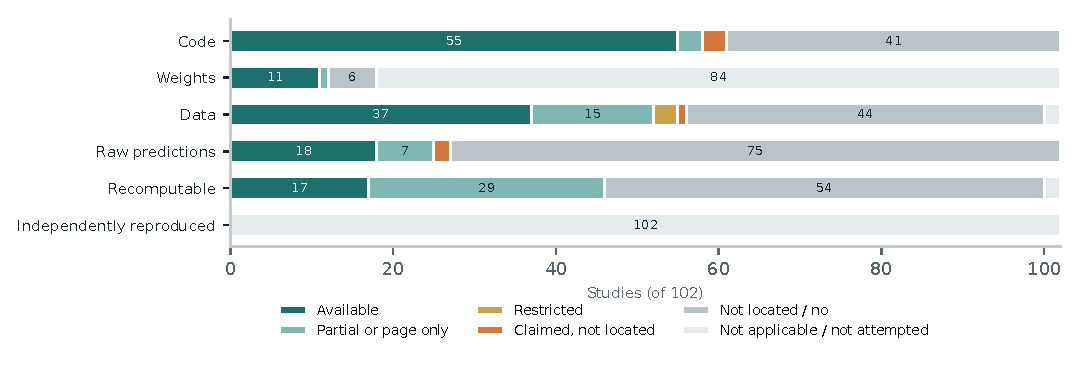
\includegraphics[width=\linewidth]{figures/openness.pdf}
\caption{Openness of the core and peripheral studies: number of studies per status in each of six independent fields.}\label{fig:openness}
\end{figure}

{\footnotesize
\begin{xltabular}{\linewidth}{>{\raggedright\arraybackslash}p{0.2\linewidth}>{\raggedright\arraybackslash}p{0.13\linewidth}>{\raggedright\arraybackslash}Xllllp{0.05\linewidth}}
\caption{Open models and readouts, read from their READMEs at pinned commits (nothing executed). “n/a”: no weights of their own, e.g. readouts of existing checkpoints; “not loc.”: not located, which is not the same as absent.}\label{tab:ecosystem}\\
\toprule
\textbf{Resource} & \textbf{Family} & \textbf{Base model} & \textbf{Weights} & \textbf{Training} & \textbf{Eval.} & \textbf{Data} & \textbf{Ref.} \\
\midrule
\endfirsthead
\toprule
\textbf{Resource} & \textbf{Family} & \textbf{Base model} & \textbf{Weights} & \textbf{Training} & \textbf{Eval.} & \textbf{Data} & \textbf{Ref.} \\
\midrule
\endhead
alperiox/\allowbreak{}audio-jevlike & Encoder decision heads & Whisper /\allowbreak{} WavLM audio encoders & not loc. & yes & yes & not loc. & \citep{gh_alperiox_audio_jevlike} \\
Contrastive-LM/\allowbreak{}CLM & Encoder decision heads & Qwen3-8B (frozen encoder) & yes & partial & partial & not loc. & \citep{gh_contrastive_lm_clm} \\
Heman10x-NGU/\allowbreak{}Verdict-open-jev & Encoder decision heads & ModernBERT (151M, GLiClass lineage) & yes & yes & yes & not loc. & \citep{gh_heman10x_ngu_verdict_open_jev} \\
hiroki-abe-58/\allowbreak{}sokudan & Encoder decision heads & sbintuitions/\allowbreak{}modernbert-ja-310m & yes & yes & yes & not loc. & \citep{gh_hiroki_abe_58_sokudan} \\
mizorewww/\allowbreak{}laya-mlx & Encoder decision heads & Laya checkpoints (ModernBERT /\allowbreak{} mmBERT) & yes & not loc. & yes & not loc. & \citep{gh_mizorewww_laya_mlx} \\
NandhaKishorM/\allowbreak{}laya & Encoder decision heads & ModernBERT-large; mmBERT-base & yes & not loc. & partial & not loc. & \citep{gh_nandhakishorm_laya} \\
olanotolu/\allowbreak{}jevbetter & Encoder decision heads & From scratch (hashed n-gram encoder) & not loc. & yes & yes & not loc. & \citep{gh_olanotolu_jevbetter} \\
SamratDuttaOfficial/\allowbreak{}WaterSheep & Encoder decision heads & answerdotai/\allowbreak{}ModernBERT-base & yes & yes & yes & not loc. & \citep{gh_samratduttaofficial_watersheep} \\
daseinlabs/\allowbreak{}open-jev & Frozen decoder option readout & Gemma 3 4B & n/\allowbreak{}a & yes & partial & not loc. & \citep{gh_daseinlabs_open_jev} \\
ekzhang/\allowbreak{}openjev-sglang & Frozen decoder option readout & Qwen3.6-35B-A3B & n/\allowbreak{}a & not loc. & partial & not loc. & \citep{gh_ekzhang_openjev_sglang} \\
featherless-ai/\allowbreak{}simple-jev & Frozen decoder option readout & Open instruction-tuned models (e.g. Gemma 4 26B-A4B) & n/\allowbreak{}a & not loc. & yes & not loc. & \citep{gh_featherless_ai_simple_jev} \\
nokia-applied-research/\allowbreak{}AnyJev & Frozen decoder option readout & any causal LM (Qwen3-8B in README) & n/\allowbreak{}a & not loc. & partial & not loc. & \citep{gh_nokia_applied_research_anyjev} \\
rorshopping/\allowbreak{}jev-on-a-laptop & Frozen decoder option readout & Stock 1.5B–8B open models & n/\allowbreak{}a & not loc. & yes & not loc. & \citep{gh_rorshopping_jev_on_a_laptop} \\
TheoLeeCJ/\allowbreak{}SemIf & Frozen decoder option readout & frozen Qwen3.5-4B and others & n/\allowbreak{}a & not loc. & partial & not loc. & \citep{gh_theoleecj_semif} \\
Yinsongxu/\allowbreak{}LLM2Jev & Frozen decoder option readout & Qwen3.5 (e.g. 4B) and other local LLMs & n/\allowbreak{}a & not loc. & yes & not loc. & \citep{gh_yinsongxu_llm2jev} \\
zhengxuyu/\allowbreak{}litjev & Frozen decoder option readout & Qwen model family & n/\allowbreak{}a & not loc. & not loc. & not loc. & \citep{gh_zhengxuyu_litjev} \\
zhihz/\allowbreak{}openjev & Frozen decoder option readout & Qwen3-4B-Instruct-2507 (frozen) & n/\allowbreak{}a & not loc. & yes & not loc. & \citep{gh_zhihz_openjev} \\
bespokelabsai/\allowbreak{}nimble & Fine-tuned decoder decision models & Qwen3.5-9B (LoRA) & yes & yes & not loc. & yes & \citep{gh_bespokelabsai_nimble} \\
FLock-io/\allowbreak{}this-that-model & Fine-tuned decoder decision models & decider-2b (Qwen3.5-2B lineage) & yes & not loc. & yes & partial & \citep{gh_flock_io_this_that_model} \\
getainode/\allowbreak{}jebadiah & Fine-tuned decoder decision models & Qwen3.8-27B, Qwen3.5-9B, Qwen3.5-4B (LoRA) & yes & yes & yes & yes & \citep{gh_getainode_jebadiah} \\
gitchw/\allowbreak{}LCT & Fine-tuned decoder decision models & Qwen2.5-0.5B, Qwen2.5-1.5B, Qwen3-8B & yes & yes & yes & yes & \citep{gh_gitchw_lct} \\
guanxuyu-sv/\allowbreak{}Visual-Jev & Fine-tuned decoder decision models & Qwen3-VL-4B & n/\allowbreak{}a & not loc. & not loc. & not loc. & \citep{gh_guanxuyu_sv_visual_jev} \\
iapp-technology/\allowbreak{}openthai-systemone & Fine-tuned decoder decision models & Qwen3.5-0.8B (continued pre-training on Thai) & yes & yes & not loc. & not loc. & \citep{gh_iapp_technology_openthai_systemone} \\
jaredpalmer/\allowbreak{}kev & Fine-tuned decoder decision models & Qwen3.5 (0.8B, 4B, 9B) & yes & yes & yes & yes & \citep{gh_jaredpalmer_kev} \\
lexmount/\allowbreak{}WebJev & Fine-tuned decoder decision models & Qwen3.5-35B-A3B-Base & yes & yes & yes & yes & \citep{gh_lexmount_webjev} \\
Mapika/\allowbreak{}decider & Fine-tuned decoder decision models & Qwen3.5-2B/\allowbreak{}4B/\allowbreak{}35B-A3B & yes & partial & not loc. & not loc. & \citep{gh_mapika_decider} \\
nico-martin/\allowbreak{}open-jev & Fine-tuned decoder decision models & Kev and DeBERTa-v3 ONNX exports & yes & not loc. & not loc. & not loc. & \citep{gh_nico_martin_open_jev} \\
OmniJev/\allowbreak{}OneJev & Fine-tuned decoder decision models & Qwen3.5-0.8B to Qwen3.8-27B (vision tower kept) & yes & yes & yes & yes & \citep{gh_omnijev_onejev} \\
OmniJev/\allowbreak{}PlayJev & Fine-tuned decoder decision models & Qwen3.5-0.8B-Base & yes & yes & not loc. & yes & \citep{gh_omnijev_playjev} \\
PsiACE/\allowbreak{}dohnuts & Fine-tuned decoder decision models & 0.8B multimodal base (LoRA) & yes & yes & yes & not loc. & \citep{gh_psiace_dohnuts} \\
Rizzo-AI-Academy/\allowbreak{}rizzo-flow & Fine-tuned decoder decision models & Spark-X2.5 4B and 1.7B (LoRA) & yes & yes & yes & not loc. & \citep{gh_rizzo_ai_academy_rizzo_flow} \\
shamazharikh/\allowbreak{}qwen-rlcd & Fine-tuned decoder decision models & Qwen3.5-0.8B & not loc. & partial & not loc. & not loc. & \citep{gh_shamazharikh_qwen_rlcd} \\
TianyuCodings/\allowbreak{}NanoJev & Fine-tuned decoder decision models & 0.6B decoder & yes & not loc. & partial & yes & \citep{gh_tianyucodings_nanojev} \\
uspraveen/\allowbreak{}Jevify & Fine-tuned decoder decision models & Gemma 4 E4B, Qwen3.5-2B/\allowbreak{}9B, Qwen3-VL-2B & yes & yes & yes & yes & \citep{gh_uspraveen_jevify} \\
Zefan-Cai/\allowbreak{}Open-Jev & Fine-tuned decoder decision models & Open-Jev 2B, 9B and 27B checkpoints & yes & yes & yes & yes & \citep{gh_zefan_cai_open_jev} \\
JoshuaSP/\allowbreak{}open-jev & Diffusion structured readout & DiffusionGemma 26B-A4B & n/\allowbreak{}a & not loc. & yes & not loc. & \citep{gh_joshuasp_open_jev} \\
mmastrac/\allowbreak{}djev & Diffusion structured readout & DiffusionGemma & n/\allowbreak{}a & not loc. & not loc. & not loc. & \citep{gh_mmastrac_djev} \\
razorback16/\allowbreak{}openjev & Diffusion structured readout & DiffusionGemma 26B-A4B & n/\allowbreak{}a & not loc. & not loc. & not loc. & \citep{gh_razorback16_openjev} \\
githubnext/\allowbreak{}localjev & Generative \& constrained adapters & DiffusionGemma via chat completions & n/\allowbreak{}a & not loc. & not loc. & not loc. & \citep{gh_githubnext_localjev} \\
typesafe-ai/\allowbreak{}system-one-adapter-python & Generative \& constrained adapters & — & n/\allowbreak{}a & not loc. & not loc. & not loc. & \citep{gh_typesafe_ai_system_one_adapter_python} \\
feder-cr/\allowbreak{}jev & — & — & not loc. & not loc. & yes & not loc. & \citep{gh_feder_cr_jev} \\
PAI-CUHK/\allowbreak{}MEDJEV & — & Qwen3 backbones (e.g. Qwen3-0.6B) & not loc. & yes & partial & not loc. & \citep{gh_pai_cuhk_medjev} \\
PAI-CUHK/\allowbreak{}SLEEPJEV & — & Polysomnography signal encoder & not loc. & yes & yes & not loc. & \citep{gh_pai_cuhk_sleepjev} \\
pCwOrM/\allowbreak{}werr & — & — & n/\allowbreak{}a & not loc. & not loc. & not loc. & \citep{gh_pcworm_werr} \\
vinnylarouge/\allowbreak{}jevlike & — & — & not loc. & yes & yes & not loc. & \citep{gh_vinnylarouge_jevlike} \\
\bottomrule
\end{xltabular}}
